\chapter{Power Management}

\begin{itemize}
    \item highlight why throttling mechanisms exist.\\
    Iccmax. first droop. maybe cite patent and/or look in the source code of edk2.
    \item cite user space idle state paper
    \item question: what uses power on the processor? (execution and memory movement)
\end{itemize}

\section{Shared Frequency Domains}
% measurements/shared-frequency-domains
Core frequencies can have an impact on other cores as shown by Schöne et al. for cores on the Alder Lake Platform which uses the same core micro-architecture as Sapphire Rappids~\cite{Schoene_2024_Alder_Lake}.
To validate that core frequencies are independent of each other, I adopt the measurement scripts from Sch\"one et al~\cite{Schoene_2024_Alder_Lake}.

For the measurement I disabled C-states, changed the cores to the lowest frequency (\SI{800}{\MHz}) and run a while true loop on one core.
The frequency of this core is measured while another core is running with turbo frequencies, either idling or also running a while true loop.
I repeated it for all combinations of cores on one socket.
No shared core frequency domains are detected, this is consitent with the previous Intel generation Skylake-SP.
\todoms{Check if I can cite the Skylake-SP here. There should be a reference in the software optimization guide.}

\section{AVX Frequencies}
\label{sec:avx-frequencies}

Starting with the Haswell Microarchitecture, Intel introduced the concept of AVX frequencies.
This allows AVX2 instructions to use a lower base and different per core turbo frequencies~\cite{Hackenberg_2015_Haswell}.
The concept is extended with a new class for AVX512 instructions for the Skylake Server Microarchitecture~\cite[Sec. 2.6.3]{Intel_Optimization_Reference_Manual_050}.
With the introduction of Ice Lake these classes are not only determined by the instruction set or register size, but a more realistic model of actual power consumption by also classifing instruction into ``Light'' and ``Heavy'' $C_{dyn}$ classes\footnote{$C_{dyn}$ describes the dynamic capacitance of instruction which is proportional to the power consumption.} by their power consumption~\cite{papazian_new_2020}.
With the addition of the AMX instruction set Intel split up these classes further ranging from ``Ultra-Light'' to ``Heavy''.
Instructions are mapped mapped to four license levels based on their instruction set and power draw.
Opportunistic AVX turbo frequencies are determined based on the classes and number of active cores.
The mapping from instruction set and power usage are displayed in~\tabref{avx-classes}~\cite{ServeTheHome_Emerald_Rapids_2023}.
In \figref{p0n-frequencies} we are able to extracte the per core opportunistic turbo frequencies per license on our testsystem using a modified version of ``intel-speed-select''.

% \begin{table}[t]
% 	\centering
% 	\caption{\label{tab:avx-classes}AVX frequency classes based on published slides from Intel.~\cite{ServeTheHome_Emerald_Rapids_2023}}
% 	\begin{tabular}{|l|c|c|c|c|}
%         \hline
%         \diagbox[height=5em]{Instruction\\Class}{\\$C_{dyn}$ Class} & 0 & 1 & 2 & 3 \\
%         \hline
%         SSE & 128 Light & 128 Heavy & & \\
%         AVX2 & 256 Light & 256 Moderate & 256 Heavy & \\
%         AVX512 & 512 Ultra-Light & 512 Light & 512 Moderate & 512 Heavy \\
%         AMX & & AMX Light & AMX Moderate & AMX Heavy \\
%         \hline \hline
%         Turbo Frequency & SSE & AVX2 & AVX512 & AMX \\
%         \hline
% 	\end{tabular}
% \end{table}

\begin{table}[bp!]
	\centering
	\caption{\label{tab:avx-classes}AVX frequency classes based on published slides from Intel.
    The $C_{dyn}$ classes 0 through 3 map to the license levels SSE, AVX2, AVX512 and AMX~\cite{ServeTheHome_Emerald_Rapids_2023}.
    The license levels that we could measure are marked in red.}
    \begin{tabular}{|l|p{0.14\textwidth}|p{0.17\textwidth}|p{0.17\textwidth}|p{0.17\textwidth}|}
        \hline
        \diagbox[width=0.24\textwidth]{$C_{dyn}$\\Class}{Instruction\\Class} & SSE & AVX2 & AVX512 & AMX \\
        \hline
        0 (SSE Frequency) & 128 Light & \cellcolor{red!15}{\textbf{256 Light}\protect\footnotemark} & 512 Ultra-Light & \\
        \hline
        1 (AVX2 Frequency) & 128 Heavy & \cellcolor{red!15}{\textbf{256 Moderate}\protect\footnotemark} & 512 Light & AMX Light \\
        \hline
        2 (AVX512 Frequency) & & 256 Heavy & \cellcolor{red!15}{\textbf{512 Moderate}\protect\footnotemark} & AMX Moderate \\
        \hline
        3 (AMX Frequency) & & & \cellcolor{red!15}{\textbf{512 Heavy}\protect\footnotemark} & AMX Heavy \\
        \hline
	\end{tabular}
\end{table}

\addtocounter{footnote}{-3}
\footnotetext[\thefootnote]{\texttt{FIRESTARTER -i 6 -\phantom{}-run-instruction-groups=REG:100}}
\addtocounter{footnote}{1}
\footnotetext[\thefootnote]{\texttt{FIRESTARTER -i 6 -\phantom{}-run-instruction-groups=REG:100,L1\_L:100}}
\addtocounter{footnote}{1}
\footnotetext[\thefootnote]{\texttt{FIRESTARTER -\phantom{}-run-instruction-groups=REG:100}}
\addtocounter{footnote}{1}
\footnotetext[\thefootnote]{\texttt{FIRESTARTER -\phantom{}-run-instruction-groups=L3\_L:100}}

Downs~\cite{Downs_2020_AVX_Downclocking} measured the influence of AVX throttling on Ice Lake by infering the license level based on the resulting frequency of the ``avx-turbo'' microarchitectural benchmark.
However he was only able to trigger two out of the three license level, leaving open the question on how instructions are mapped to ``Light'' and ``Heavy'' classes.
Laukemann et al.~\cite{laukemann_microarchitectural_2024} showed the same for Sapphire Rapids using ``likwid-bench'' with the ``peakflops\_avx512\_fma'' and ``peakflops\_avx\_fma'' microarchitectural benchmark.
They were also only able to show two out of the four license levels.
\todoms{cite avx-turbo and likwid-bench}

\begin{figure}[]
    \centering
    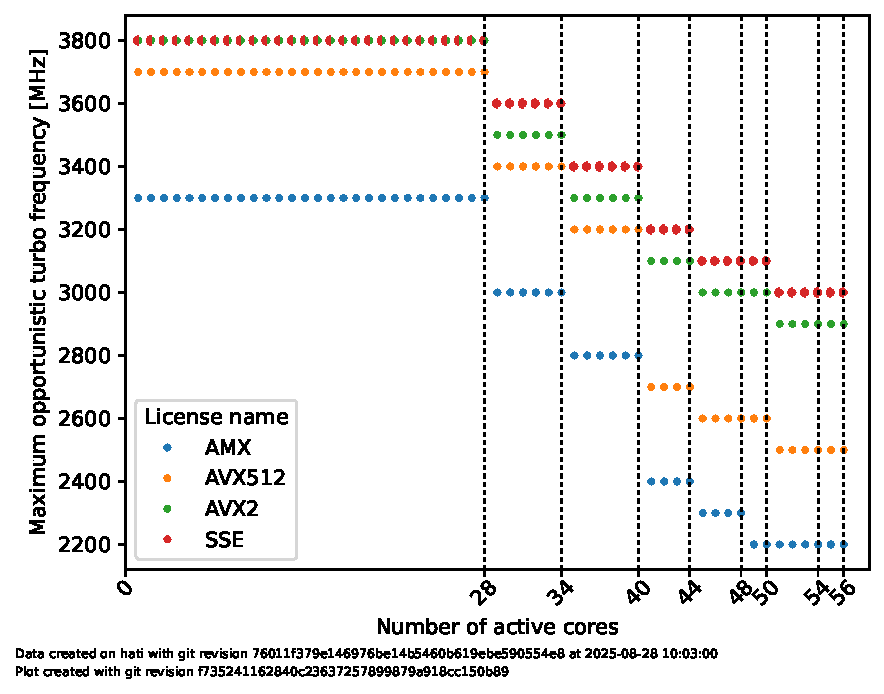
\includegraphics[width=0.8\columnwidth]{fig/avx-frequency-license-bands/avx-frequency-license-bands.pdf}
    \caption{\label{fig:p0n-frequencies}Opportunistic AVX turbo frequencies of the test system extracted using Intel Speed Select Technology.
    The number of active cores are split into eight buckets. The license and the bucket decides the resulting turbo frequency.
    In the first bucket the SSE and AVX2 license bands share the same frequency.}
\end{figure}

%Register Address: 1ADH, 429 MSR\_TURBO\_RATIO\_LIMIT
%Register Address: 1AEH, 430 MSR\_TURBO\_RATIO\_LIMIT\_CORES

To associate which events trigger the processor cores to be part of a license level, I designed a microbenchmark that executes small compute kernels on a fixed number of cores and measure the resulting core frequencies.
This methodology is fundamentaly the same as demostrated by Downs and Laukemann et al.
However, as license level can only be validated using theri maximal turbo frequency,
I ensure that the RAPL power limiting mechanisms is not triggered.
Using ``Intel Speed Select Core-Power'' I can set one core to priority group zero and all other to priority group 1 with a fixed low maximum frequency of \SI{1600}{\MHz}.
This will priorize the power draw of the core in group zero over the others.
The frequency measurement is done on the core in group zero, which should run at the maximum turbo frequency.
``Intel Speed Select'' is described in more detail in~\secref{isst}.
I prototype this measurement with four different FIRESTARTER kernels.
Each kernel is executed for \SI{60}{\s} discarding the first \SI{30}{\s} and last \SI{5}{\s}.
Hyperthreading is disabled.
The resulting opportunistic AVX frequencies are displayed in~\figref{validated-p0n-frequencies}.
The findings of~\figref{p0n-frequencies} can clearly be validated.
This also highlights that frequency class dependent opportunistic core frequencies are independant of the ``Intel Speed Select Core-Power'' mechanism.

\begin{figure}[]
    \centering
    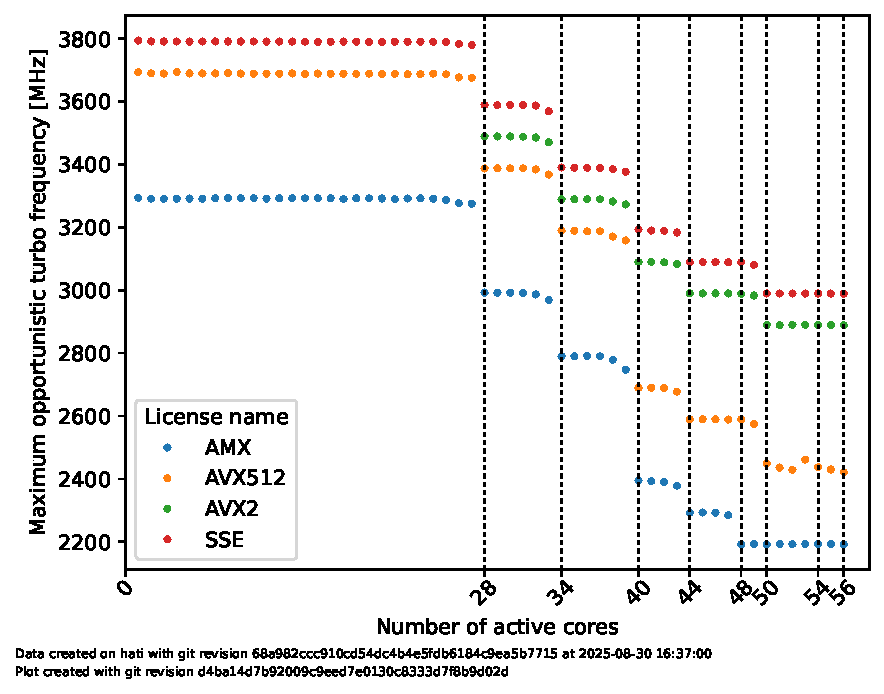
\includegraphics[width=0.8\columnwidth]{fig/avx-frequency-license-bands-validation/validate-avx-frequency-license-bands.pdf}
    \caption{\label{fig:validated-p0n-frequencies}Validation of the opportunistic AVX turbo frequencies of the test system extracted using Intel Speed Select Technology.
    The number of active cores are split into eight buckets. The license and the bucket decides the resulting turbo frequency.
    In the first bucket the SSE and AVX2 license bands share the same frequency. I ensure that the package power does not exceed the maximum of \SI{350}{\watt} TDP of the test system.}
\end{figure}

\section{AVX Frequency Anomalies}
\label{sec:avx-anomalies}

To further test the effects of AVX frequency thottling mechanisms on the processor, I ran the same four FIRESTARTER workloads as described in~\secref{avx-frequencies} without the use of ``Intel Speed Select Core-Power''.
In~\secref{avx-anomalies-low-freq} I discovered throttling of the core frequency at its lowest frequency (\SI{800}{\MHz}) when running with the AMX or AVX512 frequency level.
In~\secref{avx-anomalies-uncore-freqency} I describe an anomaly in the uncore frequency selection causing suboptimal energy efficiency for the AMX frequency level.

\subsection{Throttling at Low Frequencies}
\label{sec:avx-anomalies-low-freq}

Each FIRESTARTER kernel is executed for \SI{60}{\s} discarding the first and last \SI{5}{\s}.
I measure the uncore frequency by polling the associated MSR every \SI{10}{\ms} on CPU 0\footnote{\url{https://github.com/marenz2569/intel-uncore-freq-dumper}}.
The measurement is repeated on the cross product of following settings:
\begin{itemize}
    \item Core frequency set to \SI{800}{\MHz}, \SI{1600}{\MHz}, \SI{2000}{\MHz} and the default frequency range of \SI{800}{\MHz}--\SI{3800}{\MHz}.
    \item Uncore frequency set to \SI{800}{\MHz}, \SI{1600}{\MHz}, \SI{2500}{\MHz} and the default frequency range of \SI{800}{\MHz}--\SI{2500}{\MHz}.
\end{itemize}
\todoms{reference the appendix for all plots}

Since the FIRESTARTER kernels do not produce peak power draw, I expect that the core frequency not throttled below the nominal frequency of \SI{2}{\GHz}.
This is the case, expect for the AVX512 and AMX frequency levels at \SI{800}{\MHz} core frequency, which are throttled to just above \SI{550}{\MHz}.
This effect is shown in~\figref{avx-anomalies-low-freq}.
The severity of the effect depends on the selected uncore frequency and is worsend with a higher frequency.

\begin{figure}[]
    \centering
    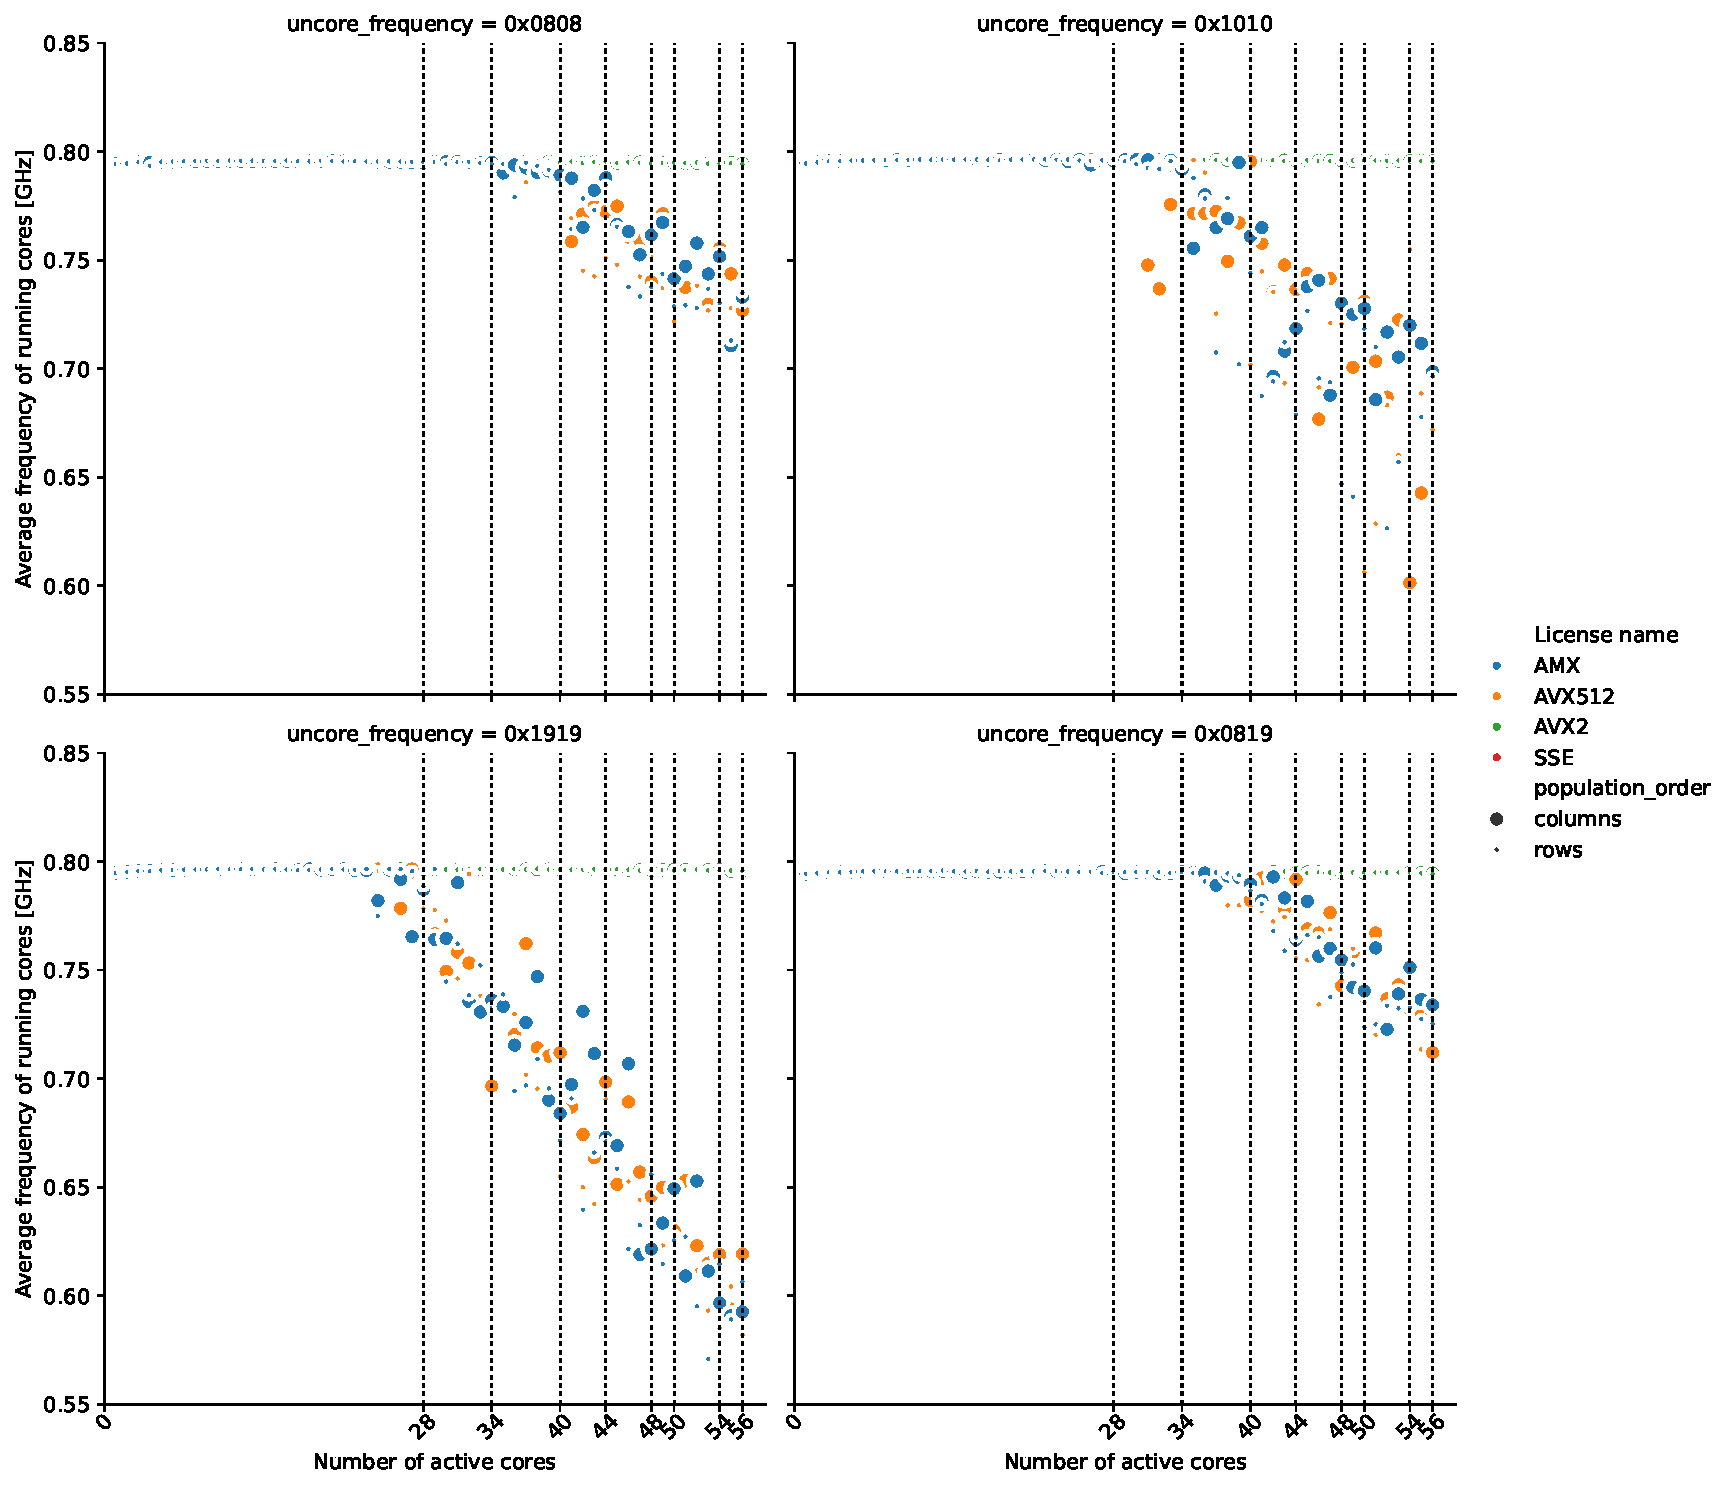
\includegraphics[width=0.8\columnwidth]{fig/avx-frequency-license-bands-without-isst-core-frequency-800.pdf}
    \caption{\label{fig:avx-anomalies-low-freq}Average core frequency across the cores running the workload with the core frequency set to \SI{800}{\MHz}. For the AMX and AVX512 frequency levels core frequency throttling below \SI{800}{\MHz} occurs.}
\end{figure}

\begin{figure}[]
    \centering
    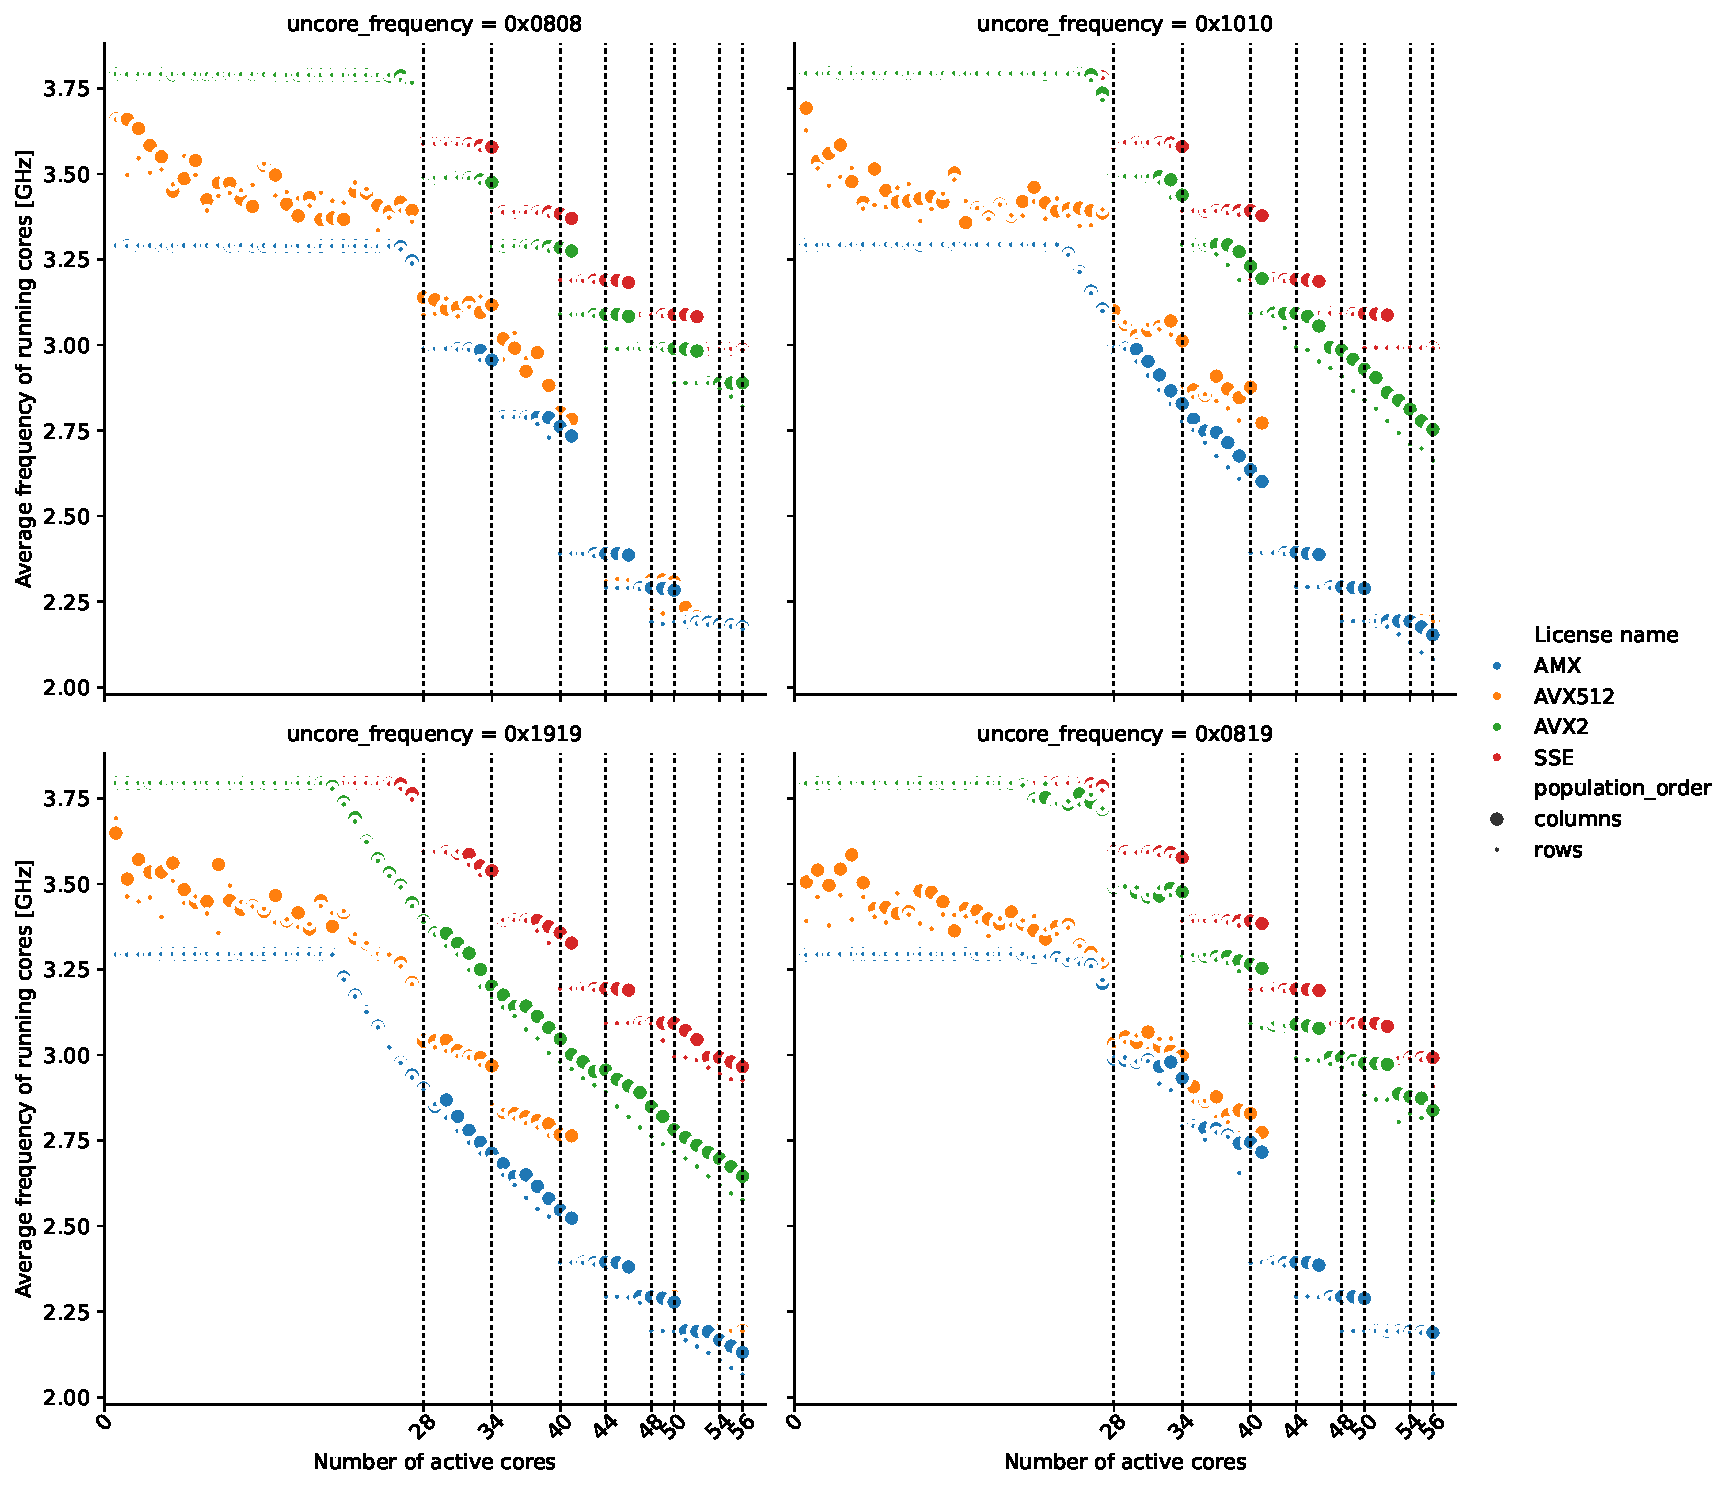
\includegraphics[width=0.8\columnwidth]{fig/avx-frequency-license-bands-without-isst-core-frequency-performance.pdf}
    \caption{\label{fig:avx-anomalies-performance}Average core frequency across the cores running the workload with no limit on the core frequency resulting in a maximal turbo frequency of \SI{3800}{\MHz}.}
\end{figure}

\subsection{Uncore Frequency Selection}
\label{sec:avx-anomalies-uncore-freqency}

I ran the four described FIRESTARTER kernels \SI{100}{} times with ``Intel Speed Select'' disabled on CPU 0--7.
CPU 8 runs the uncore frequency measurement.
Hyperthreading is disabled and the CPUs used for the measurement are isolated from OS noise with a kernel parameter\footnote{isolcpus=0-8 nohz\_full=0-8}.
Each kernel is executed for \SI{20}{\s} discarding the first \SI{10}{\s} and last \SI{2}{\s}.
I expect the same performance and power draw across all runs.
However, two different levels of power draw with the kernels runnign at the AMX frequency level are visible in~\figref{avx-frequency-uncore-anomaly-package-power-ecdf}.
This is caused by the uncore frequency selecting either \SI{1.4}{\GHz} for \SI{65}{\percent} and \SI{2.5}{\GHz} for \SI{35}{\percent} of the samples.
No major deviation of performance across the samples is observable, compare with~\figref{avx-frequency-uncore-anomaly-mean-perf}.
\figref{avx-frequency-uncore-anomaly-max-ee} show the resulting suboptimal energy efficiency reduction of more than \SI{25}{\percent} for the samples which caused a selection of the higher uncore frequency.
The SSE frequency license also shows a reduction in energy efficiency for some samples, I could however not find a specific effect causing this change with the metrics I measured.

\begin{figure}[t!]
    \subfloat[Cumulative distribution of drawn package power.]{%
        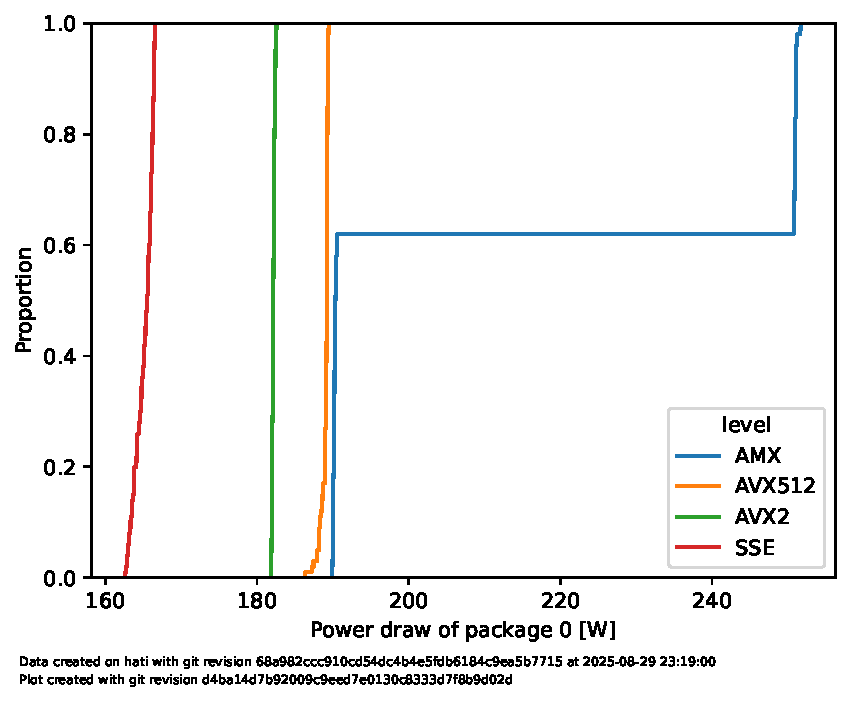
\includegraphics[width=.48\linewidth]{fig/avx-frequency-uncore-anomaly/package-power-ecdf.pdf}%
        \label{fig:avx-frequency-uncore-anomaly-package-power-ecdf}%
    }\hfill
    \subfloat[Cumulative distribution of uncore frequency.]{%
        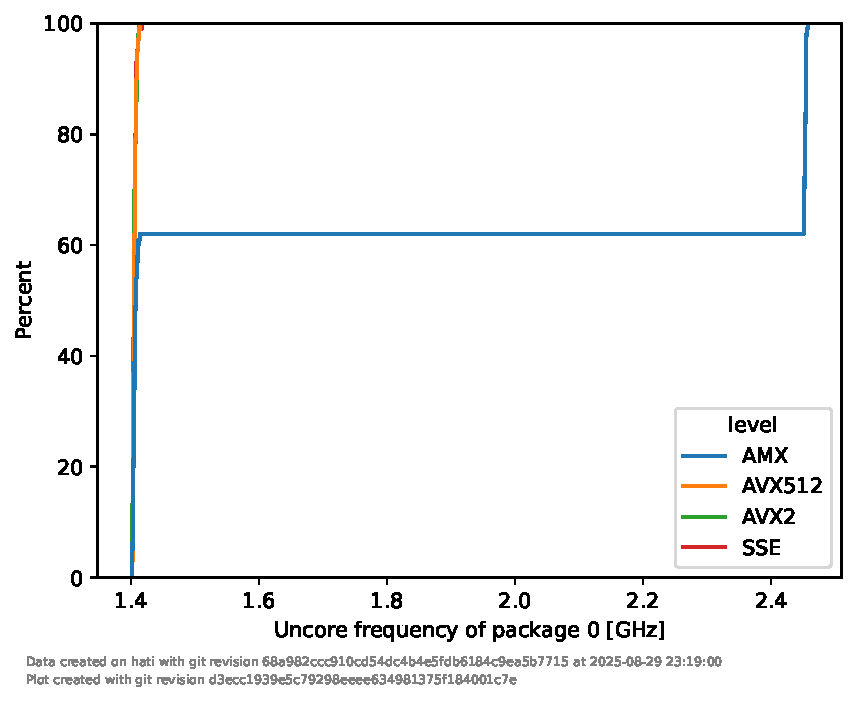
\includegraphics[width=.48\linewidth]{fig/avx-frequency-uncore-anomaly/uncore-freq-ecdf.pdf}%
        \label{fig:avx-frequency-uncore-anomaly-uncore-freq-ecdf}%
    }\\
    \subfloat[Cumulative distribution of the performance deviation relative to the mean perfomance.
    The perfomance is modeled as the number of executed instructions per second by multiplying the freqency times the nunber of executed instruction per cycle.]{%
        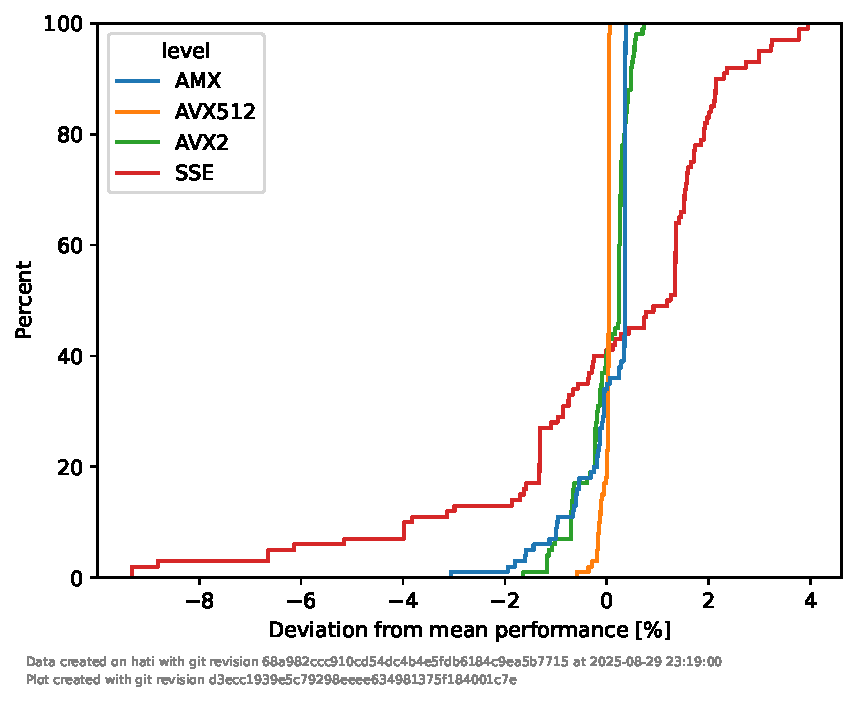
\includegraphics[width=.48\linewidth]{fig/avx-frequency-uncore-anomaly/performance-ecdf.pdf}%
        \label{fig:avx-frequency-uncore-anomaly-mean-perf}%
    }\hfill
    \subfloat[Cumulative distribution of the deviation from the maximal energy efficiency.
    The energy efficiency is modeled as the performance divided by the packager power.]{%
        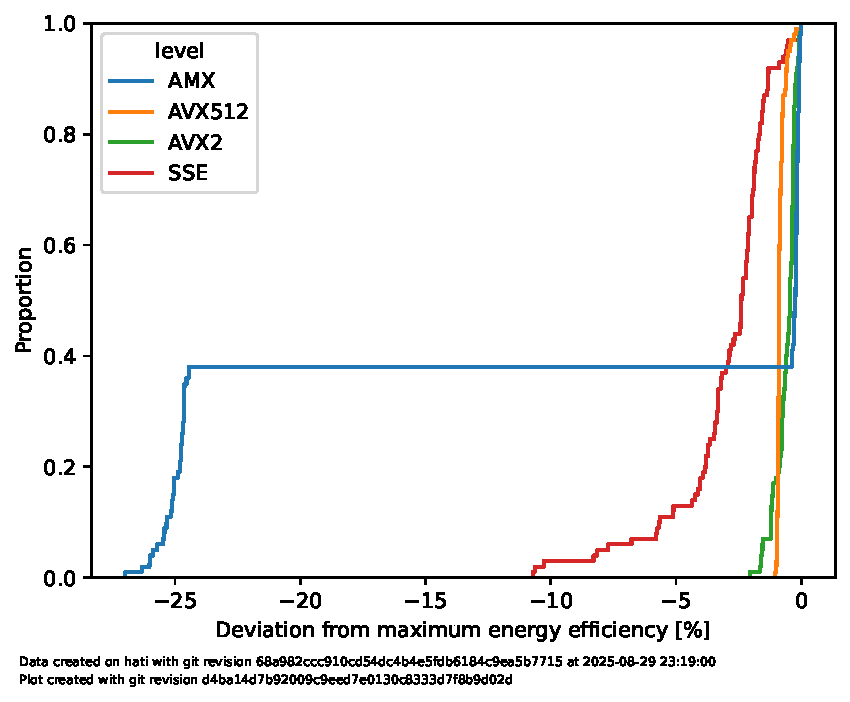
\includegraphics[width=.48\linewidth]{fig/avx-frequency-uncore-anomaly/energy-efficiency-ecdf.pdf}%
        \label{fig:avx-frequency-uncore-anomaly-max-ee}%
    }
    \caption{Metrics of the uncore frequency anomaly measurement.
    We show metrics of \SI{100}{} runs of four FIRESTARTER kernels, each triggering a different license levels, as cumulative distributions.
    \figref{avx-frequency-uncore-anomaly-package-power-ecdf} shows the increase in package power for \SI{35}{\percent} of the samples.
    This increase is caused by the increase in uncore frequency shown in~\figref{avx-frequency-uncore-anomaly-uncore-freq-ecdf}.}
    \label{fig:avx-frequency-uncore-anomaly}
\end{figure}


\section{Intel speed select}
\label{sec:isst}

\begin{itemize}
    \item intel speed select technology and avx frequencies are independent of one another.\\
    one plot to support this claim. potential for optimization on intels side.
    sort of: turbo-mode (turbo ratio limit) is one of many algorithm.
    turbo-freq buckets are another. (garanteed turbo freqs in high prio buckets, vs low prio)
    perf-profile is yet another. (different TRLs (?) and base frequencies with different number of cores)
    core-power with CLOS groups are another. (different frequency limits based on different priorities)
    base-freq
    \item open question: how do they work together?
    \item Information about Core power\cite[pages~87-111]{Intel_2021_HPM}
\end{itemize}

\todoms{what does this do. what are the CLOS groups. cite the patent. how fast are the frequency transitions of the control loop?}


\section{P-State Latencies}
\label{sec:pstate_latencies}

\todoms{Describe DVFS, latencies occur between switches, cite ftalat paper, schoene skylake and alderlake for comparison.}

To measure the latencies that occur during DVFS switches, I adapt ftalat, a benchmark developed by CITE PAPER, with modification by CITE PAPER.
ftalat measures the execution time of a compute loop with a fixed processor frequency.
The measurement methodology is as follows:
First, a frequency change is requested.
Second, the time until the execution time of the compute loop matches the expected for the requested frequency is measured.
The frequency is switched back and a random time between \SI{0}{\us} and \SI{20000}{\us} is waited before being repeated for \SI{4000}{} times.

In~\cite{Schoene_2024_Alder_Lake}, Schöne et al. demonstrated that the transition latencies for Alder Lake processors depend on the time since the last frequency transition.
I split the measurement data at a interval of \SI{1}{\ms} since the last frequency transition and plot the median latencies in~\figref{pstate_latencies_median}.
\todoms{Check}
Below this interval the behaviour is the same as in Skylake-SP~\cite{Schoene_2019_SKL} with a higher latency of \SI{600}{\us} instead of \SI{500}{\us}.
Above this interval we see a different behaviour when switching to a higher frequency of \SI{1.9}{\GHz} and above.
Latencies are generally higher in this area, with some samples showing a even higher transition latency.
In \figref{pstate_latencies_95percentQuantile} I display the 95th percentile plot for the transition latency.
This was chossen behause of many outliers probably caused by measurement noise and allow us to estimate the worst case transtion latency to between \SI{1100}{\us} and \SI{2000}{\us}.

The higher latencies depends on the time between the last frequency change, as shown in~\figref{pstate_latencies_time_dependance}.
The frequency transition from \SI{1.2}{\GHz} to \SI{1.8}{\GHz} does not display any depdency between the latency and wait time between the transtion as expected from previous processor generations.
This is consitent with testing performed on a Skylake-SP system.
For frequency transitions from \SI{1.2}{\GHz} to \SI{1.9}{\GHz} and above, we see two regions.
The first in the range of \SI{1000}{\us} and around \SI{1500}{\us}, emits the same behavour as explain above.
At around \SI{2000}{\us} we see a repeating pattern with a period of \SI{1625}{\us}, which intern contains samples which are not spread across the x-axis as previous, but are aligned with a period of \SI{200}{\us}.
Interestingly the number of samples which are above a transition latency of around \SI{900}{\us} decrease with an increase in frequency change.
Similar results have been reported by Schöne et al. for transition latencies of Alder Lake processors~\cite{Schoene_2024_Alder_Lake}.
Furthermore, most samples do not align on a specific transition latency but are spread across a region of \SI{200}{\us}.
I conclude that for the region with the higher transtion latency the mechanisms as described by Schöne et al. is not applicable~\cite{skylake_paper}.
The power management seems to have an additional mechanisms that requies a frequency change to be finished at or before \SI{200}{\us}, if this is not possible that would result in another penaly of \SI{200}{\us}.
This could be linked to external power managment that has to increase the voltage for the specific core which could be bound to such period.
Further work is required to explain the cause of the high latencies for some frequency changes.

\begin{itemize}
    \item cite Irma Esmer Papazian New 3rd Gen Intel® Xeon® Scalable Processor (Codename: Ice Lake-SP)
    \item slide 15, Core Frequency Transition block time not measured using ftalat, but removed predecessor Ice Lake-SP
\end{itemize}


\begin{figure}[]
    \begin{subfigure}[t]{0.45\linewidth}
        \centering
        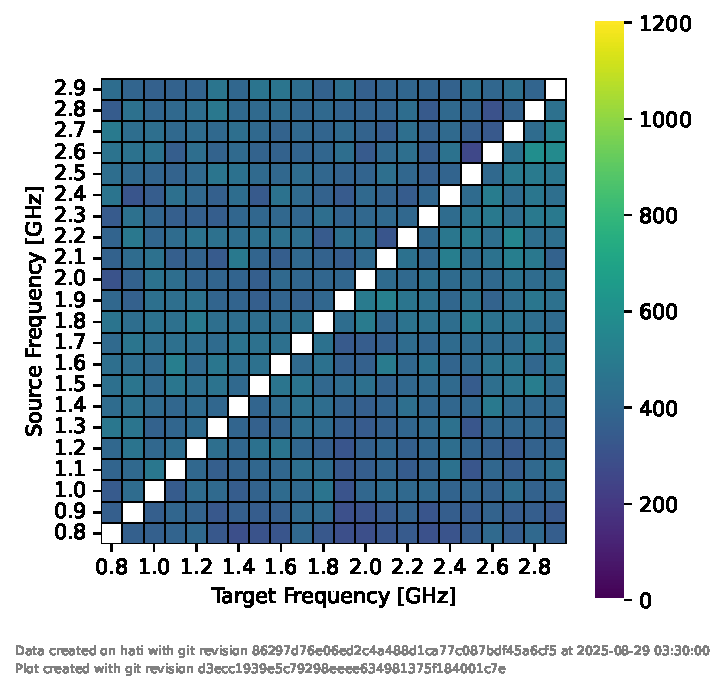
\includegraphics[width=\linewidth]{fig/ftalat/ftalat_median_<1ms_hati.pdf}
        \caption{\label{fig:pstate_latencies_median_lt_1ms}Median p-state latencies. ($< \SI{1}{\ms}$)}
    \end{subfigure}
    \hfill
    \begin{subfigure}[t]{0.45\linewidth}
        \centering
        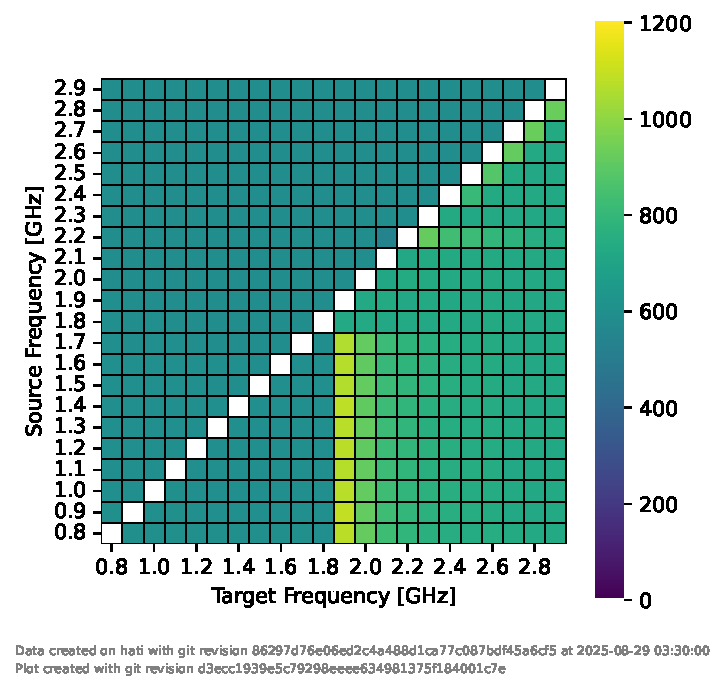
\includegraphics[width=\linewidth]{fig/ftalat/ftalat_median_>1ms_hati.pdf}
        \caption{\label{fig:pstate_latencies_median_gt_1ms}Median p-state latencies. ($> \SI{1}{\ms}$)}
    \end{subfigure}
    \caption{\label{fig:pstate_latencies_median}Median P-State switching latencies of the Sapphire Rappids processor, differentiated by wait times between frequency transitions below and above \SI{1}{\ms}.}
\end{figure}

\begin{figure}[]
    \centering
    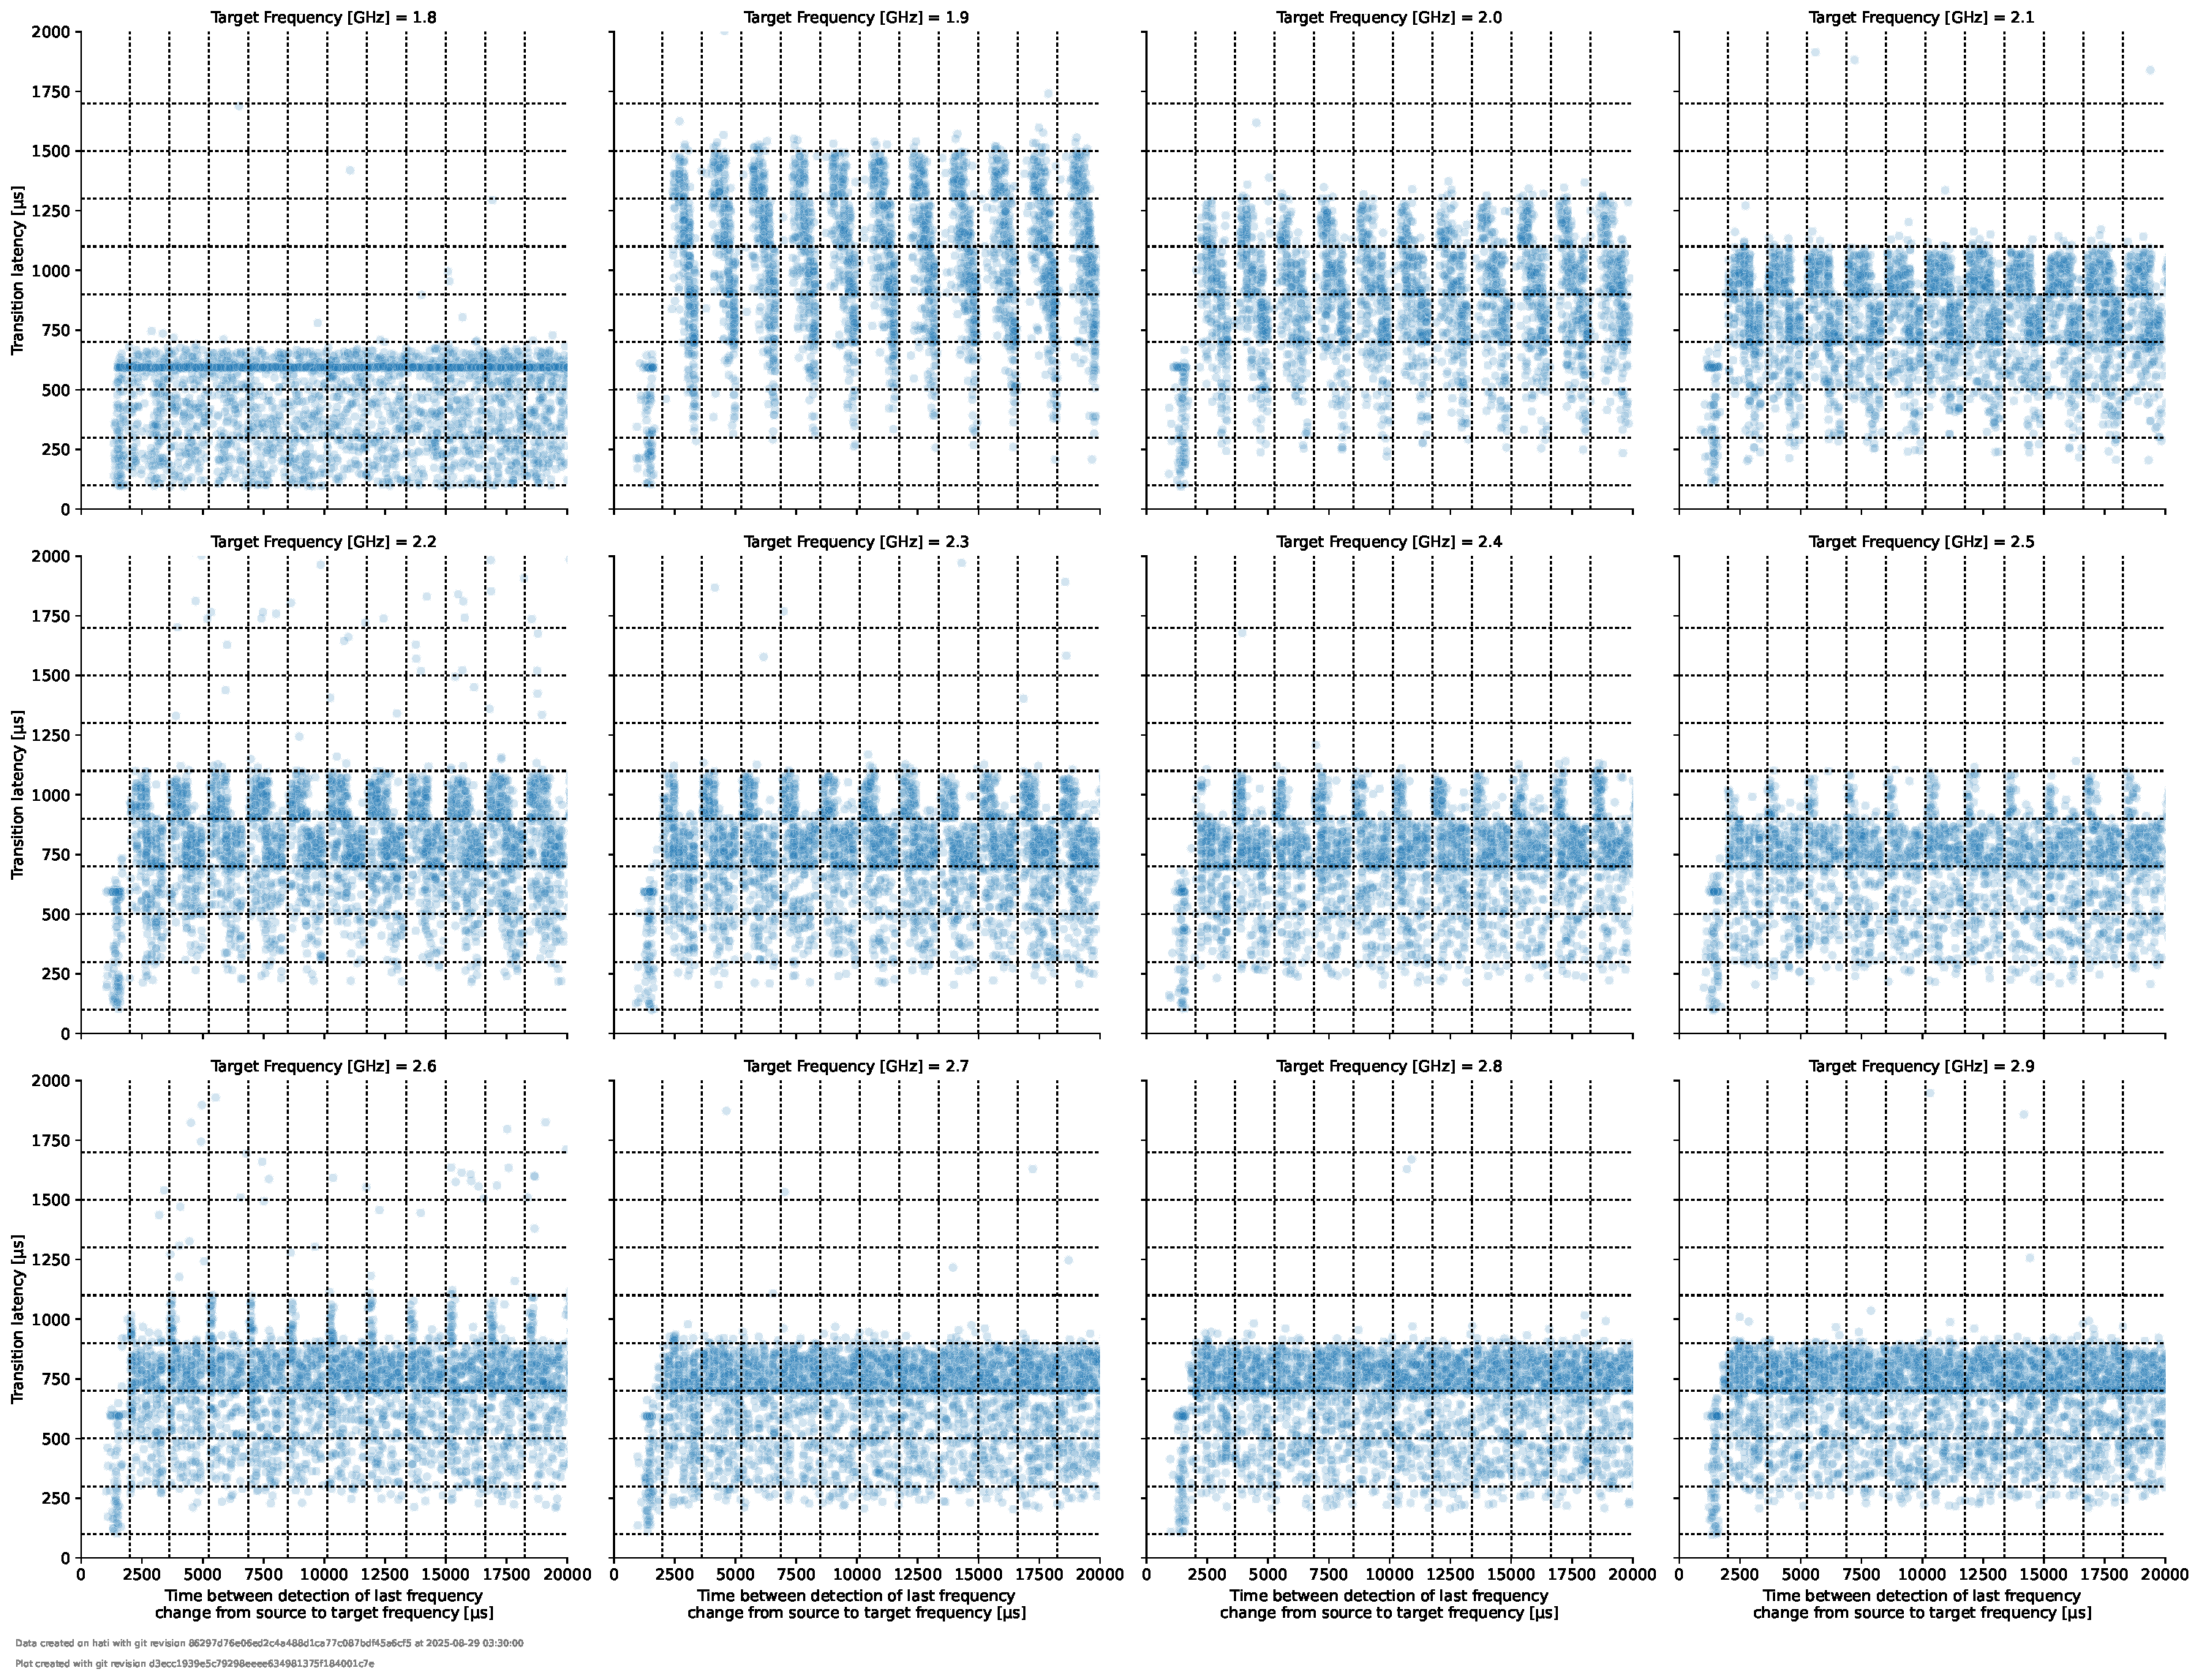
\includegraphics[width=\columnwidth]{fig/ftalat/ftalat_scatter_wait_transition_latency_hati.pdf}
    \caption{\label{fig:pstate_latencies_time_dependance}Dependance of the time between the detection events of transitions from \SI{1.2}{\GHz} to \SI{1.8}{}, \SI{1.9}{}, ..., \SI{2.9}{\GHz}. For better lines for bins of size \SI{1625}{\us} and \SI{200}{\us} have been included for the x and y-axis respectively. These plots are included for frequency transitions in~\appref{pstate_latencies_scatter_complete}}
\end{figure}

\begin{figure}[]
    \centering
    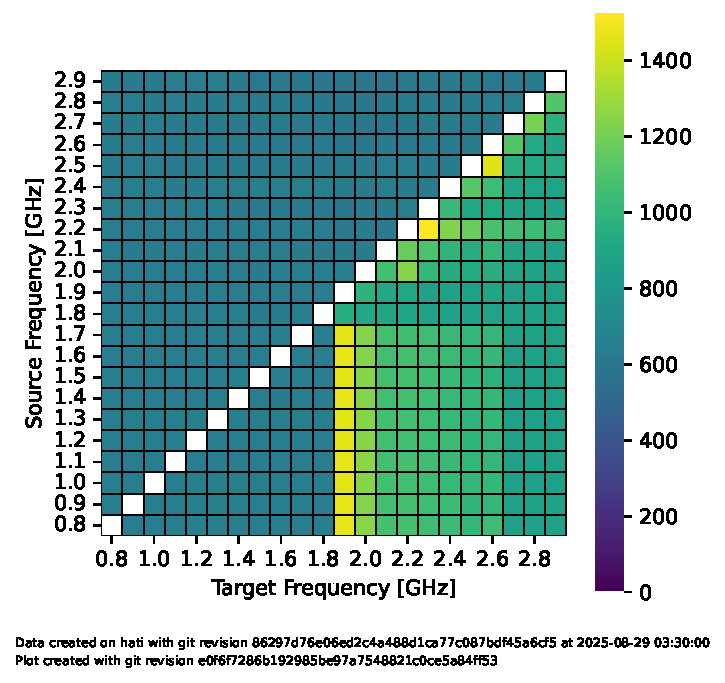
\includegraphics[width=0.45\columnwidth]{fig/ftalat/ftalat_95percentQuantile_hati.pdf}
    \caption{\label{fig:pstate_latencies_95percentQuantile}95th percentile of P-state switching latencies.}
\end{figure}


\section{Uncore Frequency Scaling}
\todoms{timing of uncore frequency change. l1 ptr, swithing to l3 ptr chasing. scripts in skylake paper.}

\begin{itemize}
    \item UFS benchmark as in Skylake paper
    \item Worst case gap latency is reduced to below \SI{8}{us}.
    \item cite Irma Esmer Papazian New 3rd Gen Intel® Xeon® Scalable Processor (Codename: Ice Lake-SP)
    \item slide 15, Mesh Frequency Transition – IO Block time reduced to 7us (validated). compared to Skylake Paper 15us.
    \item change time until the frequency is stabalized is not measured as in ftalat.
\end{itemize}


\begin{figure}[]
    \begin{subfigure}[t]{0.3\linewidth}
        \centering
        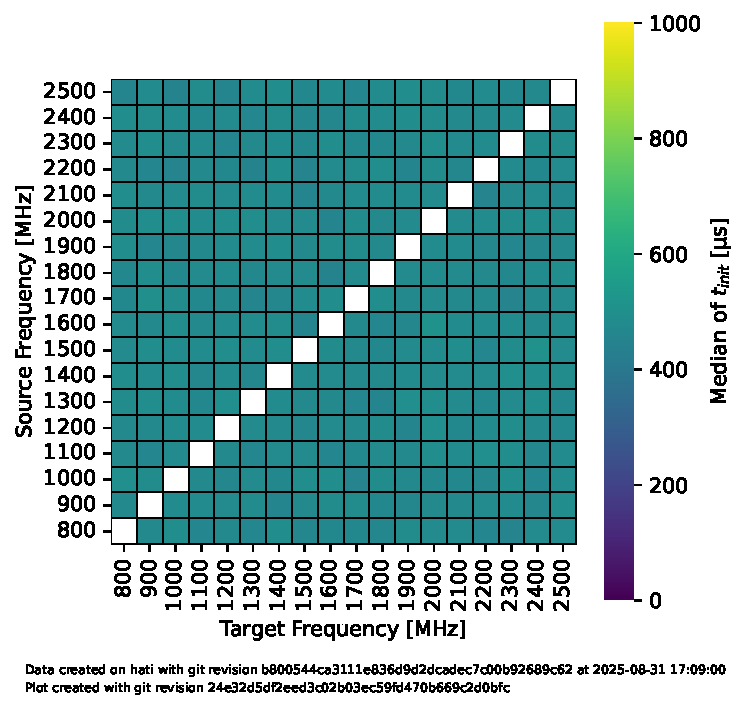
\includegraphics[width=\linewidth]{fig/uncore-frequency-switching-latency/median-t-init.pdf}
        \caption{\label{fig:a}Median time until an uncore frequency change is executed.}
    \end{subfigure}
    \hfill
    \begin{subfigure}[t]{0.3\linewidth}
        \centering
        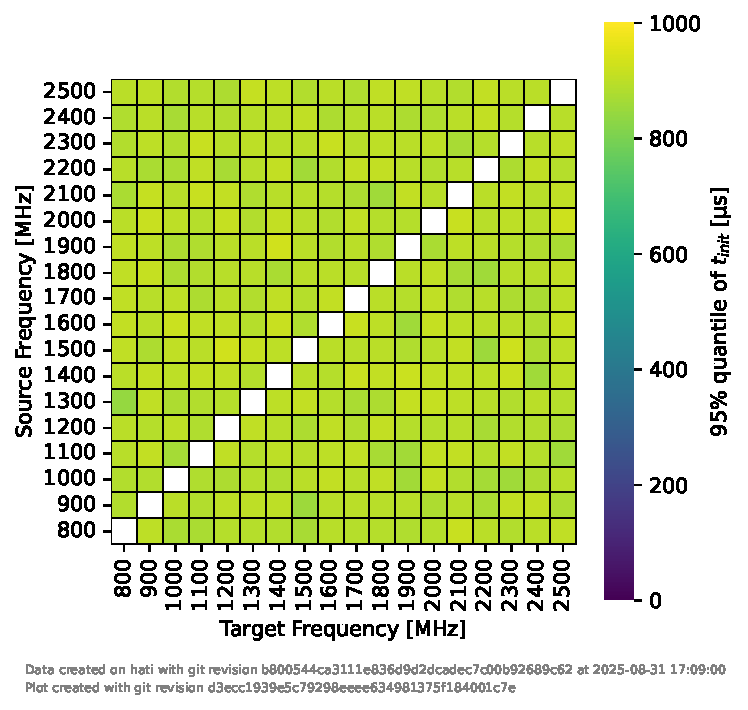
\includegraphics[width=\linewidth]{fig/uncore-frequency-switching-latency/95percentile-t-init.pdf}
        \caption{\label{fig:b}95th percentile of the time until an uncore frequency change is executed.}
    \end{subfigure}
    \hfill
    \begin{subfigure}[t]{0.3\linewidth}
        \centering
        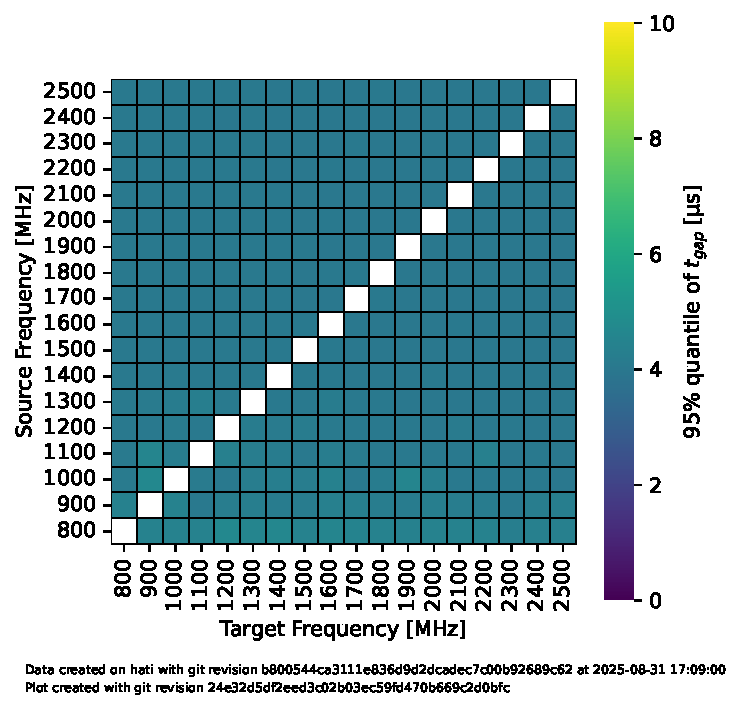
\includegraphics[width=\linewidth]{fig/uncore-frequency-switching-latency/95percentile-t-gap.pdf}
        \caption{\label{fig:b}95th percentile time the IO is blocked for the uncore frequency change.}
    \end{subfigure}
    \caption{\label{fig:c}Time until the uncore IO is blocked, after which the frequency is adjusted on the Sapphire Rappids processor.}
\end{figure}

\section{Idle State Latencies}

\begin{figure}[!ht]
    \centering
    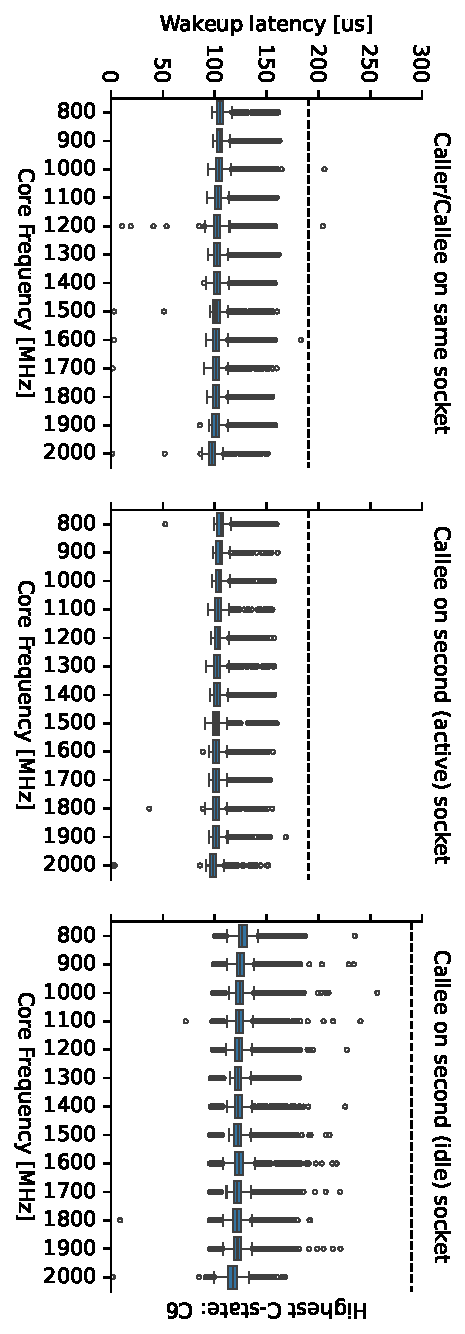
\includegraphics[width=\columnwidth]{fig/cstate-latencies/C_state_latencies.pdf}
    \caption{\label{fig:c6_latencies}C-state latency of C6 measured using methodology developed by Schöne et al.
The dotted line displays the hardcoded wakeup latency in the \protect\textbf{intel\_idle} kernel module.
\protect\footnotemark}
\end{figure}
\footnotetext{data structure \protect\textbf{spr\_cstates} in \protect\url{https://github.com/torvalds/linux/blob/72840238e2bcb8fb24cb35d8d1d5a822c04e62a4/drivers/idle/intel\_idle.c}}

\begin{itemize}
    \item Anomaly with perfomance governor at \SI{2.0}{\GHz}, C6 not used?
    \item more samples requied that in previous papers
    \item worse c-state latencies compared to Skylake
    \item explain error bars
    \item add reported c-state latencies of OS.
    \item With powersave governor c-states are set correcty (/sys/devices/system/cpu/cpu0/cpuidle/state*/time validated manually) but transition latencies are equivalent to C6.
\end{itemize}
